% !TeX root = ../main.tex

\section{Ход лабораторной работы}

\subsection{Исследование спектра и автокорреляционной функции сигнала в полосе «Бесконечность»}

Начальный этап исследований проводился в идеальных условиях радиоприёма, позволяющих исключить влияние внешних дестабилизирующих факторов. Аддитивный гауссовский шум входного тракта, гармоническая помеха и квантование отсчётов входного процесса и опорных колебаний были отключены. Полоса пропускания радиочастотного блока была установлена в значение «Бесконечность», что на практике означает ограничение спектрального диапазона исключительно частотой дискретизации модели $f_d = 51{,}1\text{ МГц}$ и теоремой Найквиста. Частотная расстройка опорного генератора несущей была задана равной нулю.

Формирование опорного дальномерного кода стандартной точности (СТ) диапазона L1 было сконфигурировано в строгом соответствии с требованиями ИКД ГЛОНАСС. Для генерации периодической псевдослучайной последовательности максимального периода (М-последовательности) длиной $N = 2^9 - 1 = 511$ тактов применён 9-разрядный регистр сдвига с линейной обратной связью (LFSR). Цепь обратной связи реализована на основе характеристического полинома $f(x) = 1 + x^5 + x^9$, определяющего суммирование по модулю 2 логических состояний 5-го и 9-го разрядов регистра с последующей подачей результата на вход первой ячейки. В исходном состоянии во все ячейки регистра записывается единичный вектор (\texttt{111111111}), а рабочий дальномерный код снимается с выхода 7-го разряда. Общий вид интерфейса модели со сконфигурированным генератором, схемой коррелятора и исходными осциллограммами представлен на рис.~\ref{fig:model_setup}.

\begin{figure}[H]
    \centering
    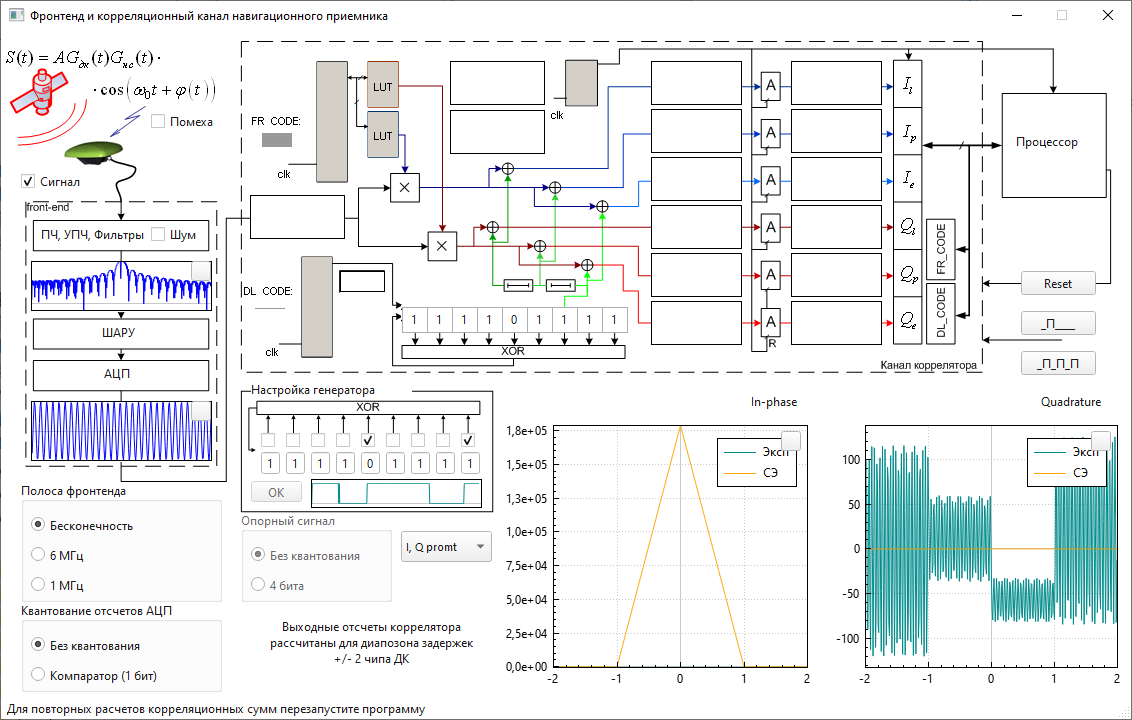
\includegraphics[width=0.85\linewidth]{1.PNG}
    \caption{Интерфейс имитационной модели коррелятора при полосе «Бесконечность»}
    \label{fig:model_setup}
\end{figure}

На выходе радиочастотного блока формируется периодический фазоманипулированный радиосигнал с прямоугольной огибающей чипов. Теоретический энергетический спектр такого процесса описывается функцией вида $\operatorname{sinc}^2(\pi f / f_c)$ с бесконечным числом затухающих боковых лепестков. График спектральной плотности мощности, полученный в окне имитационной модели для полосы «Бесконечность», представлен на рис.~\ref{fig:spec_inf}.

\begin{figure}[H]
    \centering
    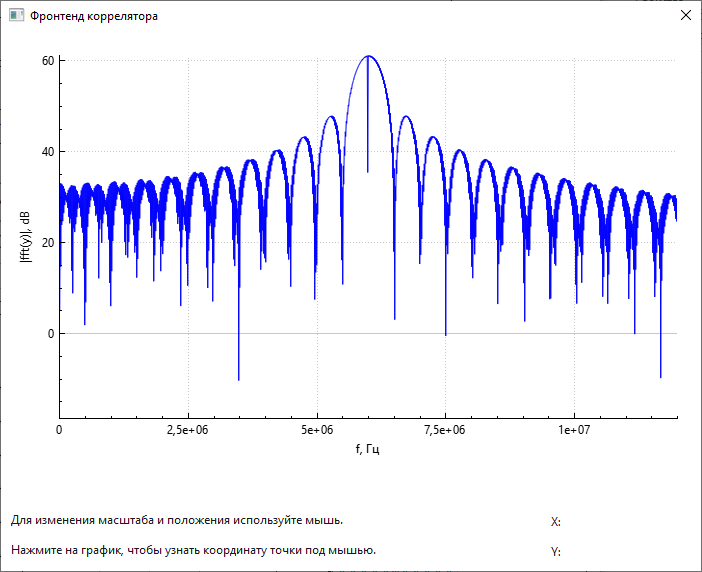
\includegraphics[width=0.68\linewidth]{2.PNG}
    \caption{Спектр радиосигнала на выходе фронтенда в полосе «Бесконечность»}
    \label{fig:spec_inf}
\end{figure}

По представленной спектральной характеристике фиксируется ярко выраженная центральная несущая гармоника на частоте $f_{if} = 6{,}0\text{ МГц}$, соответствующая установленной промежуточной частоте тракта. Границы главного лепестка спектра по первым спектральным нулям составляют $f_{left} = 5{,}489\text{ МГц}$ и $f_{right} = 6{,}511\text{ МГц}$, что даёт ширину полосы по первым нулям $\Delta f = 1{,}022\text{ МГц}$. Это значение точно равно удвоенной частоте следования чипов дальномерного кода ГЛОНАСС СТ ($2 f_c = 2 \times 511\text{ кГц} = 1{,}022\text{ МГц}$). Боковые лепестки монотонно спадают без фильтрационного среза во всей полосе анализа вплоть до границы Найквиста.

На рис.~\ref{fig:corr_inf_clean} представлены графики вычисленных корреляционных сумм как функции разности задержек дальномерного кода сигнала и опорных колебаний для идеальных условий.

\begin{figure}[H]
    \centering
    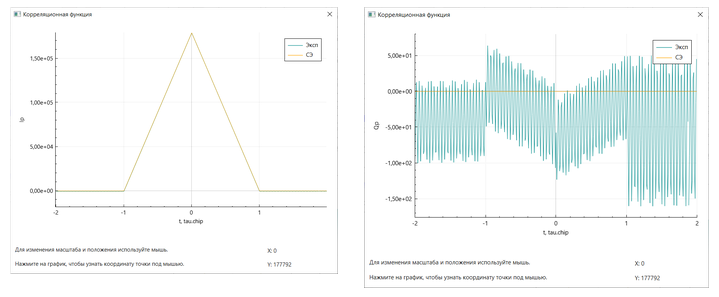
\includegraphics[width=1\linewidth]{1_corr.png}
    \caption{Спектр радиосигнала на выходе фронтенда в полосе «Бесконечность»}
    \label{fig:corr_inf_clean}
\end{figure}

Анализ графиков подтверждает теоретические ожидания. Синфазная составляющая \(I_p\) (рис.~\ref{fig:corr_inf_clean}, а) образует эталонный треугольный пик автокорреляционной функции с острым изломом в точке \(\Delta\tau = 0\) и шириной основания ровно в два периода чипа (от \(-1\) до \(+1\) чипа). Амплитуда главного пика достигает значения \(1{,}78 \times 10^5\) отн. ед., полностью повторяя ход кривой статистического эквивалента. 






\subsection{Исследование влияния полосы пропускания фронтенда и группового времени запаздывания}

Сравнительный анализ показывает, что фильтр с полосой \(6\text{ МГц}\) пропускает центральный и несколько ближайших боковых лепестков спектра ПСП (рис.~\ref{fig:spec_6mhz}). На графике синфазной компоненты \(I_p\) видно, что треугольная вершина начинает сглаживаться, а экстремум функции смещается в область запаздывания в точку \(\Delta\tau_{chip} \approx 0{,}293\text{ мкс}\) (рис.~\ref{fig:corr_6mhz}). Перераспределение фазы в фильтре вызывает также появление отклика в квадратурном канале \(Q_p\), максимум которого сдвинут на аналогичную величину.

\begin{figure}[H]
    \centering
    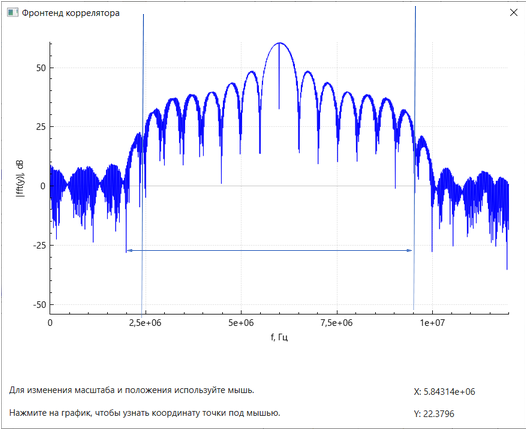
\includegraphics[width=0.7\linewidth]{6_spec.PNG} % Спектр для 6 МГц
    \caption{Спектр сигнала при полосе пропускания фронтенда 6 МГц}
    \label{fig:spec_6mhz}
\end{figure}

\begin{figure}[H]
    \centering
    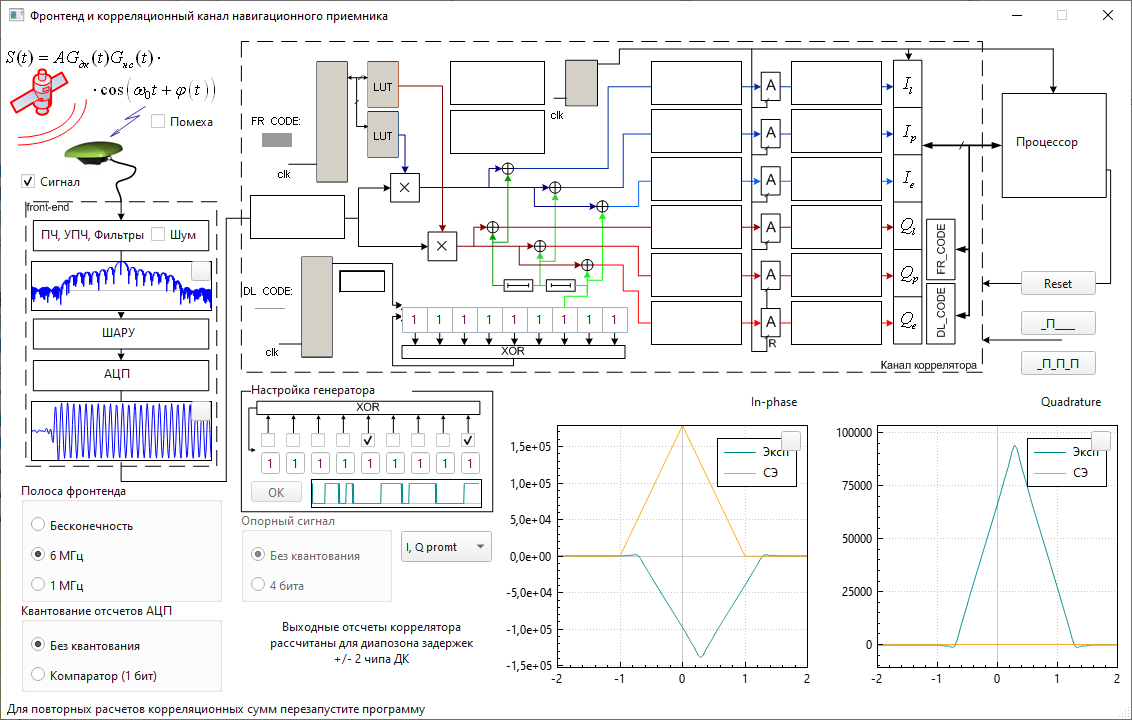
\includegraphics[width=0.7\linewidth]{3.PNG} % Корреляция для 6 МГц
    \caption{Корреляционные функции при полосе пропускания фронтенда 6 МГц}
    \label{fig:corr_6mhz}
\end{figure}

При сужении полосы тракта до \(1\text{ МГц}\) фильтр становится уже ширины главного лепестка сигнала ГЛОНАСС СТ (\(\Delta f_{main} = 1{,}022\text{ МГц}\)). Происходит резкая деформация спектрального профиля: подавляются не только боковые лепестки, но и срезаются периферийные участки основного лепестка (рис.~\ref{fig:spec_1mhz}). В полосе \(1\text{ МГц}\) вершина корреляционного отклика полностью утрачивает остроту: корреляционный всплеск сильно расплывается, а его склоны становятся пологими (рис.~\ref{fig:corr_1mhz}). Падение крутизны склонов снижает коэффициент передачи дискриминатора схемы слежения за задержкой (ССЗ), повышая флуктуационную ошибку слежения за кодом. Задержка распространения огибающей возрастает более чем в четыре раза, смещая положение максимума функции в точку \(\Delta\tau_{chip} \approx 1{,}455\text{ мкс}\).

\begin{figure}[H]
    \centering
    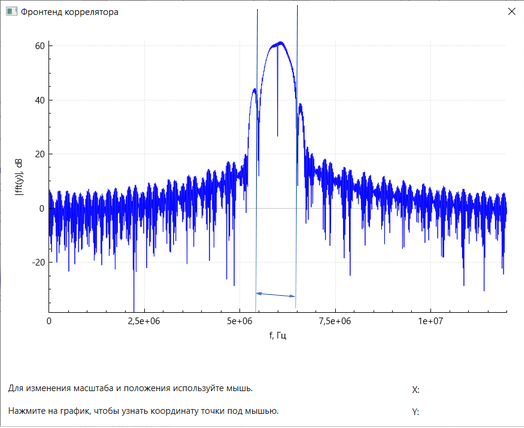
\includegraphics[width=0.7\linewidth]{1_spec.PNG} % Спектр для 1 МГц
    \caption{Спектр сигнала при полосе пропускания фронтенда 1 МГц}
    \label{fig:spec_1mhz}
\end{figure}

\begin{figure}[H]
    \centering
    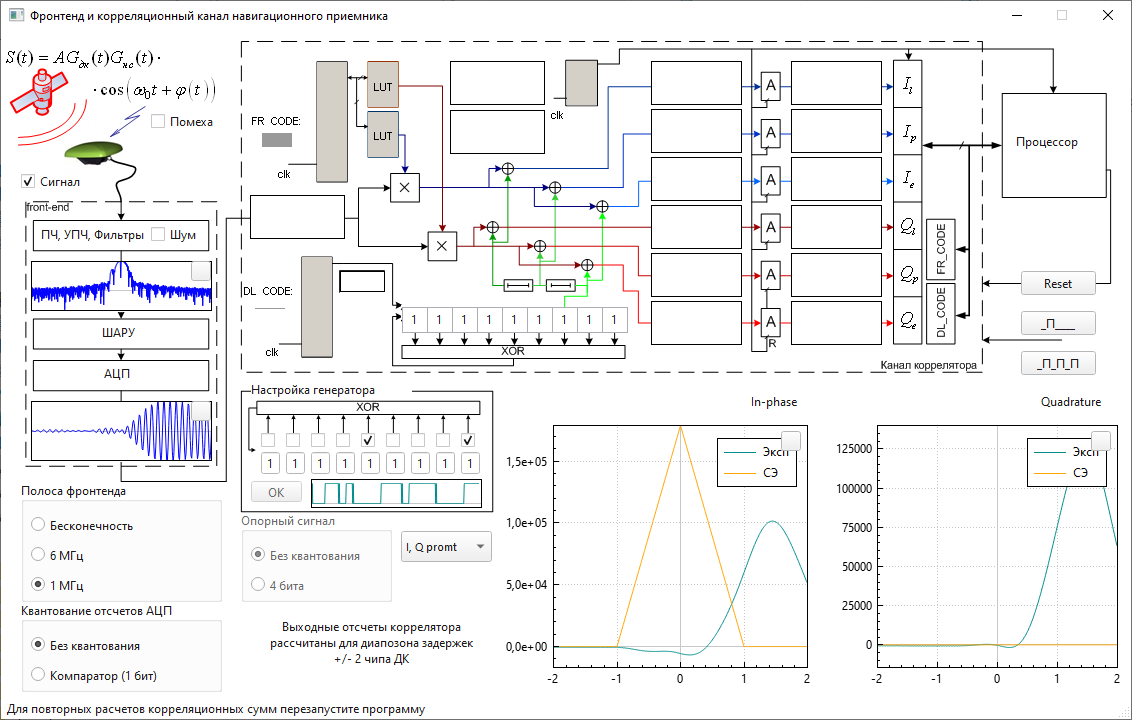
\includegraphics[width=0.7\linewidth]{4.PNG} % Корреляция для 1 МГц
    \caption{Корреляционные функции при полосе пропускания фронтенда 1 МГц}
    \label{fig:corr_1mhz}
\end{figure}

Физической причиной наблюдаемого временного смещения корреляционного пика является наклон фазочастотной характеристики аналогового фильтра. Прохождение узкополосного процесса через реактивные цепи сопровождается групповым временем запаздывания \(\tau_{\text{гр}} = -d\varphi(\omega)/d\omega\). По графикам корреляционных функций (рис.~\ref{fig:corr_6mhz} и рис.~\ref{fig:corr_1mhz}) можно напрямую оценить величину смещения вершины пика. Для полосы \(6\text{ МГц}\) групповое время запаздывания составляет \(\tau_{\text{гр}} = 0{,}29\text{ мкс}\). При сужении полосы до \(1\text{ МГц}\) запаздывание значительно возрастает и составляет \(\tau_{\text{гр}} = 1{,}45\text{ мкс}\).

Сводные результаты анализа влияния полосы аналогового тракта на геометрию корреляционного пика и задержку сведены в табл.~\ref{tab:frontend_res}.

\begin{table}[H]
\centering
\caption{Влияние полосы фронтенда на параметры корреляционного пика}
\label{tab:frontend_res}
\small
\begin{tabular}{|c|c|p{5cm}|}
\hline
\textbf{Полоса} & \textbf{Задержка \(\tau_{\text{гр}}\), мкс} & \textbf{Характер геометрии пика АКФ} \\ \hline
\(\infty\) & \(0{,}00\) & Симметричный треугольник с острым изломом \\ \hline
\(6\text{ МГц}\) & \(0{,}29\) & Умеренно сглаженный купол с сохранением крутизны \\ \hline
\(1\text{ МГц}\) & \(1{,}45\) & Пологий расширенный купол с низкой крутизной \\ \hline
\end{tabular}
\end{table}











\subsection{Исследование шумовых характеристик и оценка отношения сигнал/шум}

Для исследования шумовых свойств коррелятора была установлена номинальная полоса пропускания фронтенда $6\text{ МГц}$. На первом шаге в отсутствие аддитивного шума была зафиксирована осциллограмма неискаженного полезного радиосигнала на интервале от $0$ до $5\text{ мкс}$ (рис.~\ref{fig:sig_clean}).

\begin{figure}[H]
    \centering
    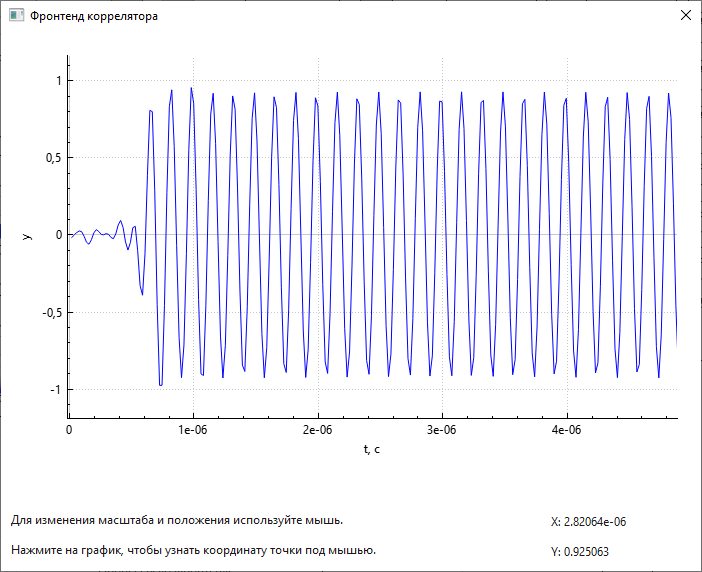
\includegraphics[width=0.7\linewidth]{5.PNG}
    \caption{Осциллограмма реализации полезного сигнала на входе АЦП}
    \label{fig:sig_clean}
\end{figure}

По представленной временной реализации гармонического сигнала амплитуда квазигармонического заполнения составляет \(A_s \approx 0{,}9\text{ В}\). Средняя мощность полезного сигнала на единичном сопротивлении рассчитывается по соотношению:
\begin{equation}
    P_s = \frac{A_s^2}{2} \approx \frac{0{,}9^2}{2} = 0{,}4\text{ Вт}.
\end{equation}

Далее полезный сигнал был отключен и введен аддитивный широкополосный шум приёмного устройства. На рис.~\ref{fig:noise_points} приведена осциллограмма шума с точками фиксации пиковых экстремумов.

\begin{figure}[H]
    \centering
    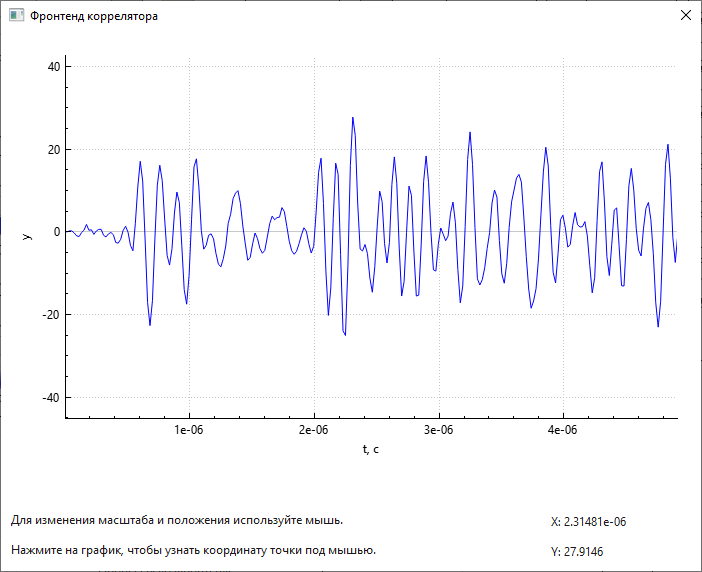
\includegraphics[width=0.7\linewidth]{6_шум точки.PNG}
    \caption{Реализация собственного шума приёмника с фиксацией экстремума}
    \label{fig:noise_points}
\end{figure}

Определим одностороннюю спектральную плотность шума. По осциллограмме размах шума по правилу трех сигм составляет:
\begin{equation}
    6\sigma_n \approx 60 \implies \sigma_n \approx 10\text{ В} - \text{СКО шума}.
\end{equation}
Тогда дисперсия шума:
\begin{equation}
    D_n = \sigma_n^2 = 100\text{ В}^2.
\end{equation}
Период дискретизации:
\begin{equation}
    T_d = \frac{1}{F_d} = \frac{1}{51{,}1 \times 10^6} = 19{,}569 \times 10^{-9} = 19{,}569\text{ нс}.
\end{equation}
Связь дисперсии и спектральной плотности для цифрового тракта:
\begin{equation}
    D_n = \frac{N_0}{2T_d} \implies N_0 = 2D_nT_d = 2 \cdot 100 \cdot 19{,}569 \times 10^{-9} = 3{,}914 \times 10^{-6}\text{ В}^2/\text{Гц}.
\end{equation}

Определим отношение мощности сигнала к односторонней спектральной плотности шума:
\begin{equation}
    q_{c/n0} = \frac{P_s}{N_0 \Delta f_\phi} = \frac{0{,}4}{3{,}914 \times 10^{-6} \cdot 6 \times 10^6} = 0{,}017.
\end{equation}
В логарифмическом масштабе:
\begin{equation}
    q_{c/n0} [\text{дБГц}] = 10 \lg(q_{c/n0}) = 10 \lg(0{,}017) = -17{,}7\text{ дБГц}.
\end{equation}


\begin{figure}[H]
    \centering
    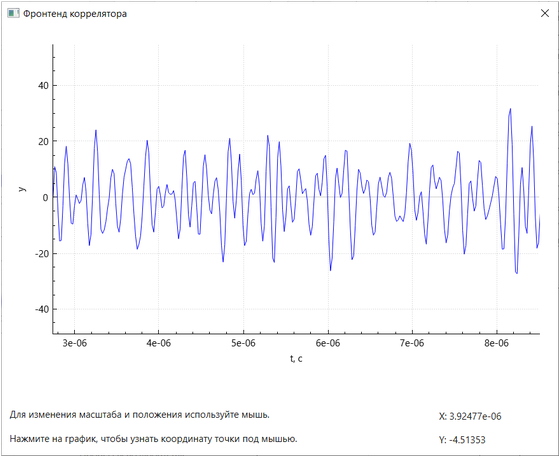
\includegraphics[width=0.7\linewidth]{2_3_sig.png}
    \caption{Реализация сигнала и шума}
    \label{fig:sig}
\end{figure}

На рис.~\ref{fig:corr_noise_6mhz} представлены вычисленные корреляционные функции сигнала в присутствии аддитивного белого гауссовского шума для синфазного ($I_p$) и квадратурного ($Q_p$) каналов при полосе пропускания $6\text{ МГц}$.

\begin{figure}[H]
    \centering
    \begin{minipage}[b]{0.48\textwidth}
        \centering
        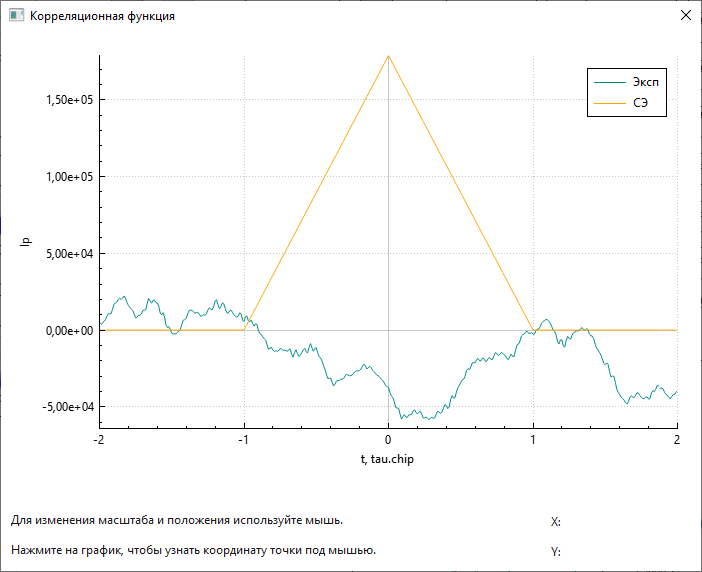
\includegraphics[width=\linewidth]{11_корплюсшум.PNG}
        \caption*{(а) Синфазная компонента $I_p$ при шуме}
    \end{minipage}
    \hfill
    \begin{minipage}[b]{0.48\textwidth}
        \centering
        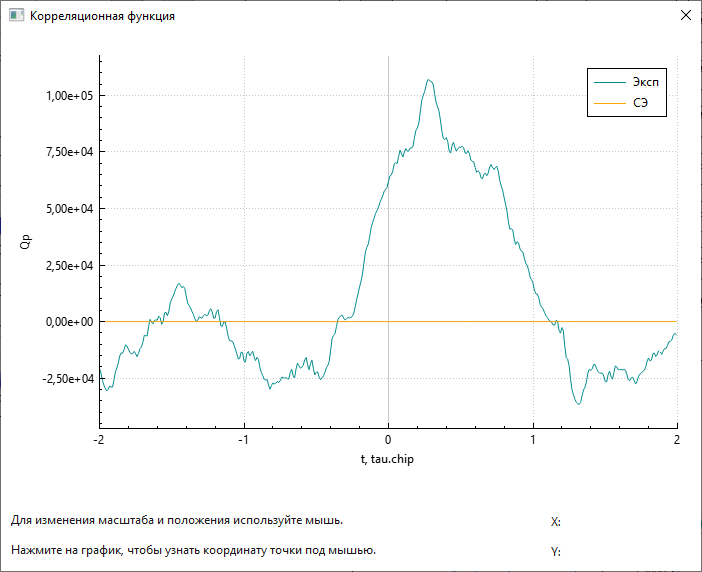
\includegraphics[width=\linewidth]{12_корплюсшум.PNG}
        \caption*{(б) Квадратурная компонента $Q_p$ при шуме}
    \end{minipage}
    \caption{Корреляционные функции смеси сигнала и шума при полосе фронтенда 6 МГц}
    \label{fig:corr_noise_6mhz}
\end{figure}

\subsection{Исследование зависимости мощности шумовой составляющей от полосы фронтенда}

В соответствии с указаниями методического пособия было проведено сравнительное исследование шумовых процессов при различных полосах избирательного тракта: «Бесконечность», \(6\text{ МГц}\) и \(1\text{ МГц}\). В полосе «Бесконечность» спектр процесса ограничен лишь частотой Найквиста, вследствие чего спектральная плотность мощности шума равномерно распределена по всей шкале анализа вплоть до \(25{,}55\text{ МГц}\). Осциллограмма входного процесса характеризуется наибольшим среднеквадратическим размахом за счет интеграции шума во всей полосе тракта.

При сужении полосы тракта до \(6\text{ МГц}\) и \(1\text{ МГц}\) спектральный пьедестал шума за пределами полосы пропускания фильтра спадает более чем на \(30\text{ дБ}\). Это приводит к существенному уменьшению дисперсии мгновенных значений процесса на входе коррелятора. Сводные результаты наблюдений за изменением шумовой составляющей корреляционных функций при изменении полосы фронтенда представлены на рисунках ниже.

% --- СТРОКА 1: СПЕКТРЫ ---
\begin{figure}[H]
    \centering
    \begin{minipage}[b]{0.32\textwidth}
        \centering
        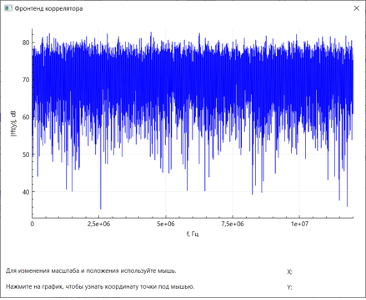
\includegraphics[width=\linewidth]{inf1.png}
        \caption*{Полоса \(\infty\)}
    \end{minipage}\hfill
    \begin{minipage}[b]{0.32\textwidth}
        \centering
        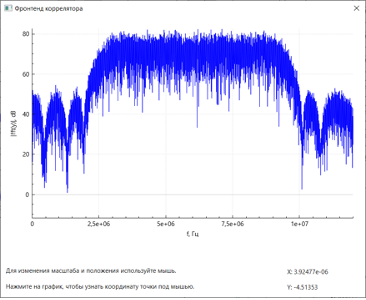
\includegraphics[width=\linewidth]{61.png}
        \caption*{Полоса 6 МГц}
    \end{minipage}\hfill
    \begin{minipage}[b]{0.32\textwidth}
        \centering
        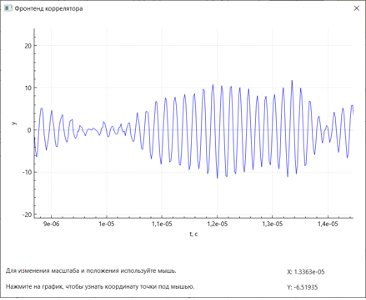
\includegraphics[width=\linewidth]{12.png}
        \caption*{Полоса 1 МГц}
    \end{minipage}
    \caption{Спектр}
    \label{fig:table_spec}
\end{figure}

% --- СТРОКА 2: РЕАЛИЗАЦИИ СИГНАЛА И ШУМА ---
\begin{figure}[H]
    \centering
    \begin{minipage}[b]{0.32\textwidth}
        \centering
        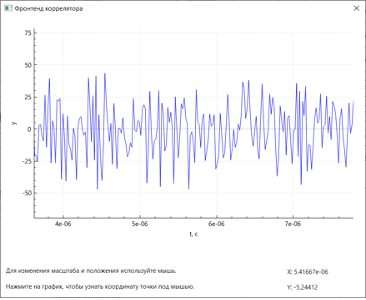
\includegraphics[width=\linewidth]{inf2.png}
        \caption*{Полоса \(\infty\)}
    \end{minipage}\hfill
    \begin{minipage}[b]{0.32\textwidth}
        \centering
        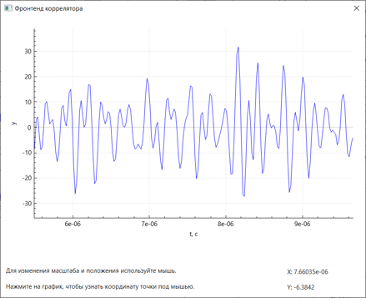
\includegraphics[width=\linewidth]{62.png}
        \caption*{Полоса 6 МГц}
    \end{minipage}\hfill
    \begin{minipage}[b]{0.32\textwidth}
        \centering
        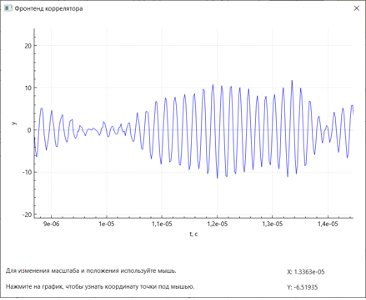
\includegraphics[width=\linewidth]{12.png}
        \caption*{Полоса 1 МГц}
    \end{minipage}
    \caption{Реализации сигнала и шума}
    \label{fig:table_sig}
\end{figure}

% --- СТРОКА 3: СИНФАЗНАЯ КОРРЕЛЯЦИОННАЯ СУММА ---
\begin{figure}[H]
    \centering
    \begin{minipage}[b]{0.32\textwidth}
        \centering
        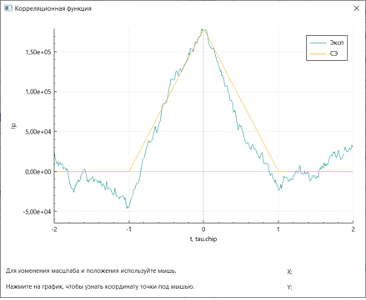
\includegraphics[width=\linewidth]{inf3.png}
        \caption*{Полоса \(\infty\)}
    \end{minipage}\hfill
    \begin{minipage}[b]{0.32\textwidth}
        \centering
        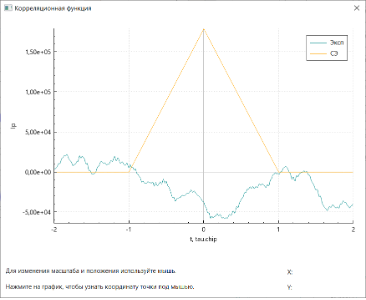
\includegraphics[width=\linewidth]{63.png}
        \caption*{Полоса 6 МГц}
    \end{minipage}\hfill
    \begin{minipage}[b]{0.32\textwidth}
        \centering
        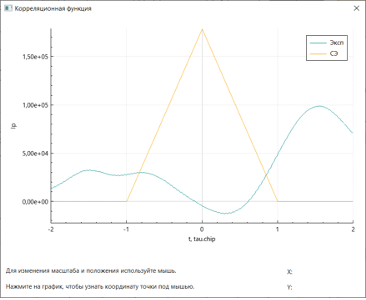
\includegraphics[width=\linewidth]{13.png}
        \caption*{Полоса 1 МГц}
    \end{minipage}
    \caption{Синфазная корреляционная сумма}
    \label{fig:table_corr_I}
\end{figure}

% --- СТРОКА 4: КВАДРАТУРНАЯ КОРРЕЛЯЦИОННАЯ СУММА ---
\begin{figure}[H]
    \centering
    \begin{minipage}[b]{0.32\textwidth}
        \centering
        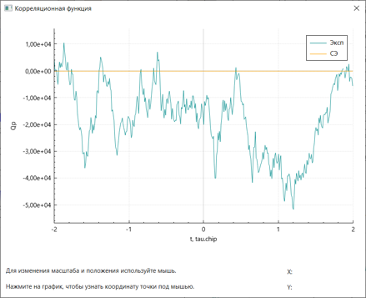
\includegraphics[width=\linewidth]{inf4.png}
        \caption*{Полоса \(\infty\)}
    \end{minipage}\hfill
    \begin{minipage}[b]{0.32\textwidth}
        \centering
        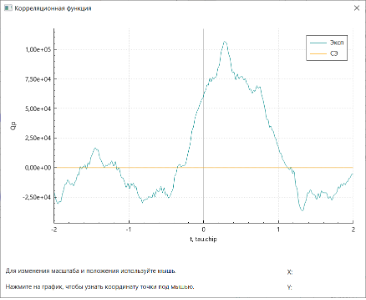
\includegraphics[width=\linewidth]{64.png}
        \caption*{Полоса 6 МГц}
    \end{minipage}\hfill
    \begin{minipage}[b]{0.32\textwidth}
        \centering
        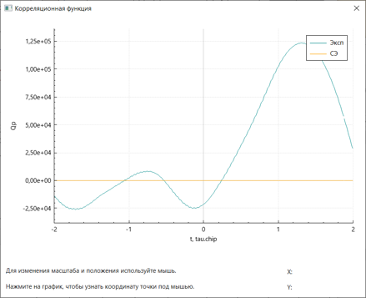
\includegraphics[width=\linewidth]{14.png}
        \caption*{Полоса 1 МГц}
    \end{minipage}
    \caption{Квадратурная корреляционная сумма}
    \label{fig:table_corr_Q}
\end{figure}

Анализ экспериментальных зависимостей показывает, что мощность шумовой составляющей на входе коррелятора прямо пропорциональна эквивалентной полосе пропускания фильтра промежуточной частоты: \(P_n = N_0 \cdot \Delta F_f\). За счет максимальной полосы пропускания (в случае «Бесконечность») треугольный пик сохраняет острую геометрию вершины, однако шумовая дисперсия на склонах АКФ оказывается наибольшей из-за отсутствия фильтрации внеполосных компонент.

При сужении полосы до \(6\text{ МГц}\) и \(1\text{ МГц}\) уровень высокочастотных флуктуаций шума на корреляционных кривых заметно снижается. Однако из-за срезания спектра полезного дальномерного кода происходит потеря крутизны дискриминационной характеристики и затягивание вершины АКФ, а также появляется фазовое запаздывание фильтра, смещающее максимум корреляционной функции.




















\subsection{Исследование зависимости мощности шумовой составляющей от полосы фронтенда}

В соответствии с дальнейшими указаниями методического пособия было проведено сравнительное исследование шумовых процессов при различных полосах избирательного тракта: «Бесконечность», $6\text{ МГц}$ и $1\text{ МГц}$. В полосе «Бесконечность» спектр процесса ограничен лишь частотой Найквиста, вследствие чего спектральная плотность мощности шума равномерно распределена по всей шкале анализа до $25{,}55\text{ МГц}$ (рис.~\ref{fig:noise_inf_spec}). Осциллограмма входного процесса, приведённая на рис.~\ref{fig:noise_inf_osc}, характеризуется наибольшим среднеквадратическим размахом за счёт интеграции шума во всей полосе тракта.

\begin{figure}[H]
    \centering
    \begin{minipage}[b]{0.48\textwidth}
        \centering
        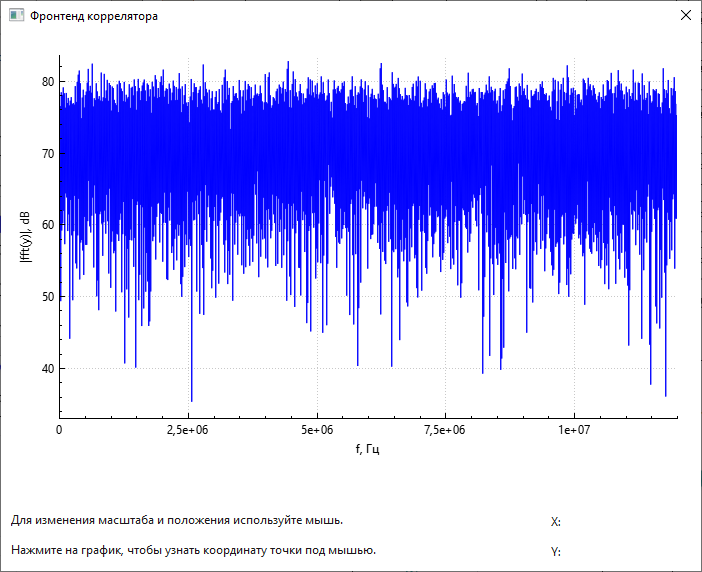
\includegraphics[width=\linewidth]{15_бескшум.PNG}
        \caption*{(а) Спектр мощности}
    \end{minipage}
    \hfill
    \begin{minipage}[b]{0.48\textwidth}
        \centering
        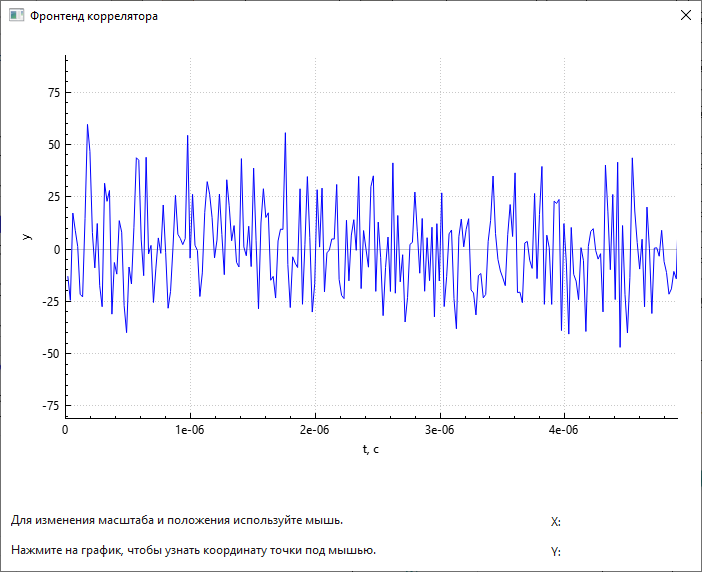
\includegraphics[width=\linewidth]{16_бескшум.PNG}
        \caption*{(б) Временная реализация}
    \end{minipage}
    \caption{Спектральные и временные характеристики шумового процесса в полосе «Бесконечность»}
    \label{fig:noise_inf_spec}
    \label{fig:noise_inf_osc}
\end{figure}

На рис.~\ref{fig:corr_inf_noise} показаны корреляционные суммы, сформированные в полосе «Бесконечность» при включенном источнике шума. За счёт максимальной полосы пропускания треугольный пик сохраняет острую геометрию вершины, однако шумовая дисперсия на склонах АКФ оказывается наибольшей из-за отсутствия фильтрации внеполосных компонент.

\begin{figure}[H]
    \centering
    \begin{minipage}[b]{0.48\textwidth}
        \centering
        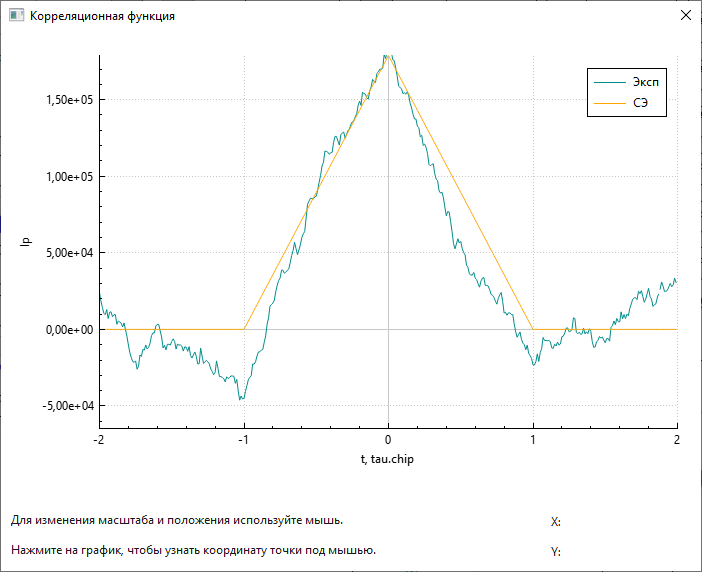
\includegraphics[width=\linewidth]{17_спплюсшумбеск.PNG}
        \caption*{(а) Синфазная компонента $I_p$}
    \end{minipage}
    \hfill
    \begin{minipage}[b]{0.48\textwidth}
        \centering
        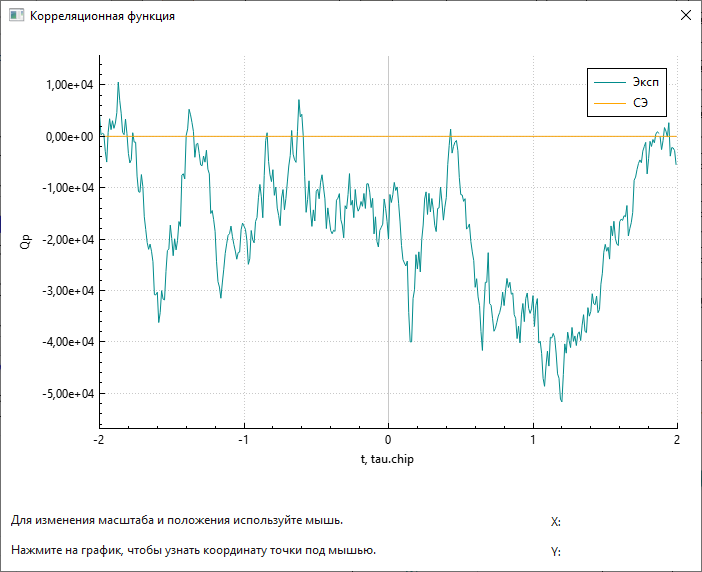
\includegraphics[width=\linewidth]{18_спплюсшумбеск.PNG}
        \caption*{(б) Квадратурная компонента $Q_p$}
    \end{minipage}
    \caption{Корреляционные функции в полосе «Бесконечность» при действии шума}
    \label{fig:corr_inf_noise}
\end{figure}

При сужении полосы тракта до $1\text{ МГц}$ спектральный пьедестал шума за пределами полосы пропускания фильтра спадает более чем на $30\text{ дБ}$ (рис.~\ref{fig:noise_1mhz_spec}). Это приводит к существенному уменьшению дисперсии мгновенных значений процесса на входе коррелятора, что отражается на осциллограмме смеси сигнала и шума (рис.~\ref{fig:noise_1mhz_osc}), где амплитудный размах колебаний уменьшается до величин порядка единиц вольт.

\begin{figure}[H]
    \centering
    \begin{minipage}[b]{0.48\textwidth}
        \centering
        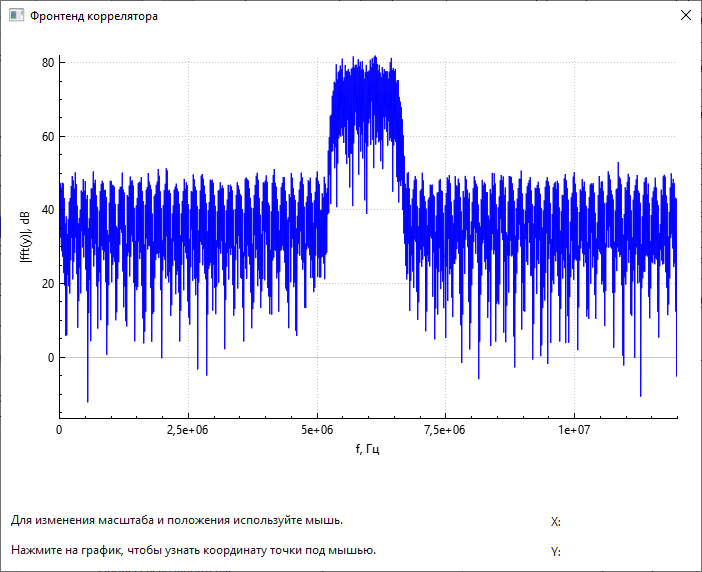
\includegraphics[width=\linewidth]{19_спплюсшум1.PNG}
        \caption*{(а) Спектр мощности при полосе 1 МГц}
    \end{minipage}
    \hfill
    \begin{minipage}[b]{0.48\textwidth}
        \centering
        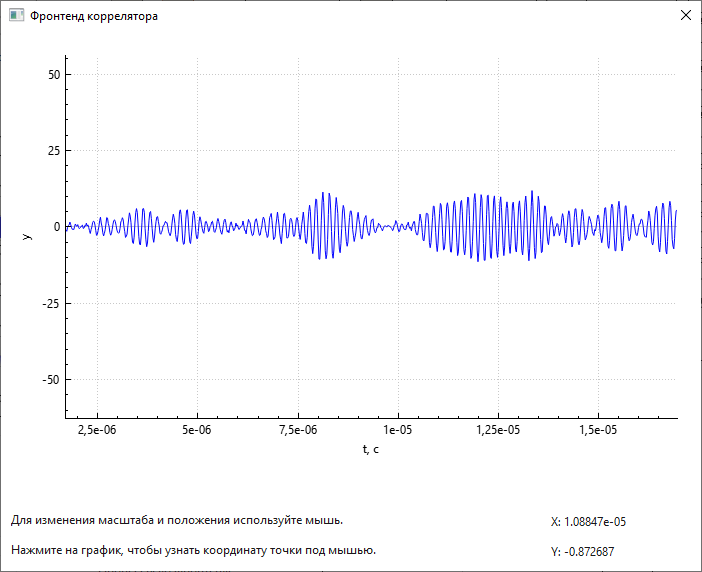
\includegraphics[width=\linewidth]{20_сигплюсшум1.PNG}
        \caption*{(б) Временная реализация смеси}
    \end{minipage}
    \caption{Характеристики сигнала и шума на выходе фронтенда при сужении полосы до 1 МГц}
    \label{fig:noise_1mhz_spec}
    \label{fig:noise_1mhz_osc}
\end{figure}

На рис.~\ref{fig:corr_noise_1mhz} приведены графики синфазной и квадратурной корреляционных сумм для полосы фронтенда $1\text{ МГц}$ при воздействии шума. Из-за значительного сужения полосы фильтрации уровень высокочастотных флуктуаций шума на кривой заметно снижается, однако пик автокорреляционной функции оказывается существенно сглаженным и сдвинутым в область задержек $\Delta\tau \approx 1{,}45\text{ чипа}$ вследствие фазового запаздывания фильтра.

\begin{figure}[H]
    \centering
    \begin{minipage}[b]{0.48\textwidth}
        \centering
        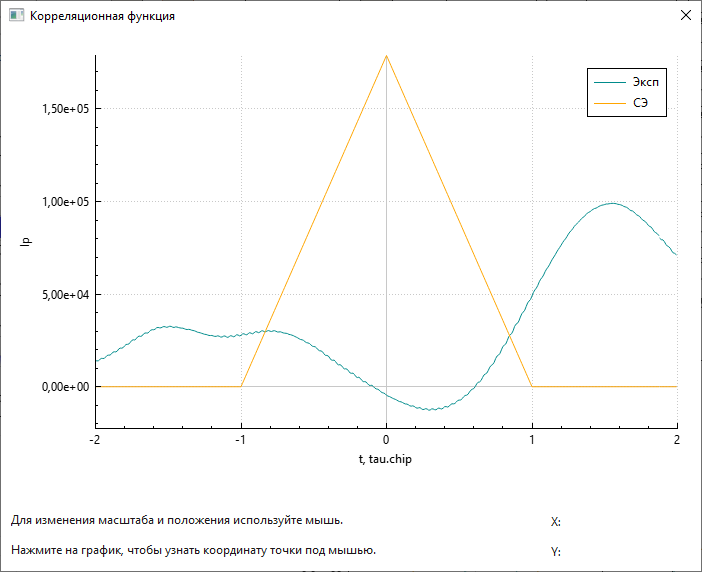
\includegraphics[width=\linewidth]{21_корплюсшум1.PNG}
        \caption*{(а) Синфазная компонента $I_p$}
    \end{minipage}
    \hfill
    \begin{minipage}[b]{0.48\textwidth}
        \centering
        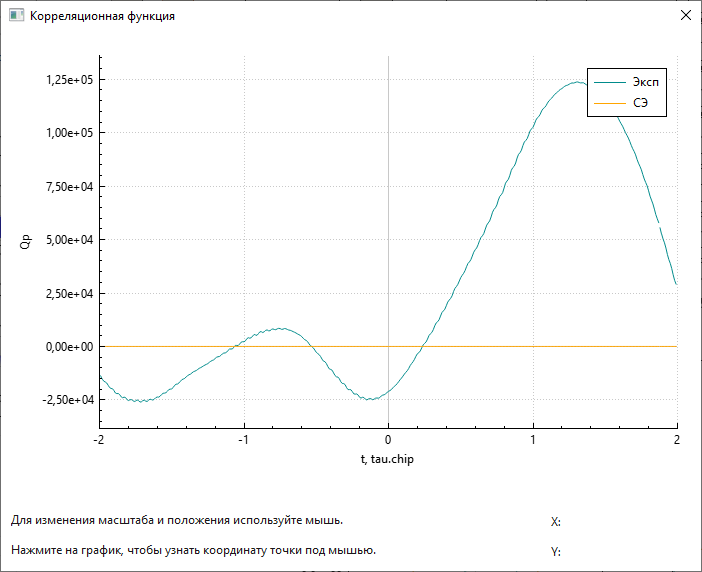
\includegraphics[width=\linewidth]{22_корплюсшум1.PNG}
        \caption*{(б) Квадратурная компонента $Q_p$}
    \end{minipage}
    \caption{Корреляционные функции сигнала в шуме при полосе фронтенда 1 МГц}
    \label{fig:corr_noise_1mhz}
\end{figure}

Анализ экспериментальных зависимостей показывает, что мощность шумовой составляющей на входе коррелятора прямо пропорциональна эквивалентной полосе пропускания фильтра промежуточной частоты: $P_n = N_0 \cdot \Delta F_f$. Сужение полосы с $\infty$ до $1\text{ МГц}$ уменьшает полную мощность шума на входе АЦП, однако из-за срезания спектра полезного дальномерного кода происходит потеря крутизны дискриминационной характеристики и затягивание вершины АКФ.

















% \subsection{Исследование влияния однобитного квантования входных отсчетов}
% 
% Для анализа влияния аналого-цифрового преобразования на работоспособность коррелятора во фрейме квантования отсчетов АЦП был активирован режим однобитного компаратора. В данном режиме входная аналоговая смесь преобразуется в бинарный поток отсчетов со значениями из множества $\{-1; +1\}$ в зависимости от знака мгновенного напряжения входного процесса. На рис.~\ref{fig:quant_osc} приведена осциллограмма квантованного сигнала в полосе «Бесконечность».
% 
% \begin{figure}[H]
    % \centering
    % 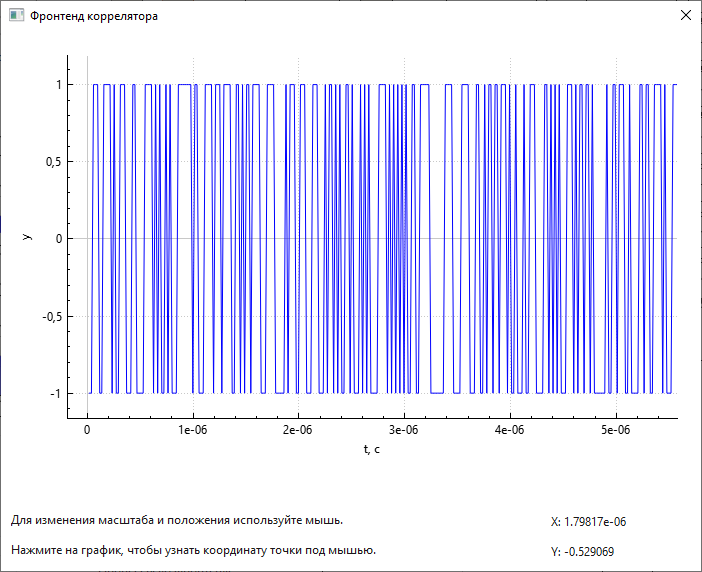
\includegraphics[width=0.7\linewidth]{23_квантбеск.PNG}
    % \caption{Осциллограмма сигнала на выходе однобитного компаратора}
    % \label{fig:quant_osc}
% \end{figure}
% 
% В отсутствие аддитивного шума однобитное квантование чистого квазигармонического фазоманипулированного сигнала приводит к нелинейному преобразованию синусоидального заполнения в периодическую последовательность прямоугольных импульсов типа «меандр». На рис.~\ref{fig:quant_corr_inf} показаны результирующие корреляционные функции при полосе «Бесконечность».
% 
% \begin{figure}[H]
    % \centering
    % \begin{minipage}[b]{0.48\textwidth}
        % \centering
        % 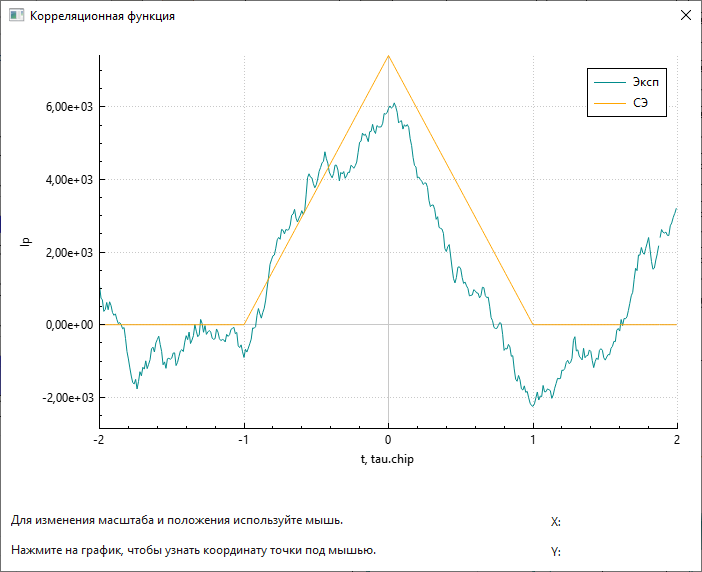
\includegraphics[width=\linewidth]{24_квантбесккор.PNG}
        % \caption*{(а) Синфазная компонента $I_p$}
    % \end{minipage}
    % \hfill
    % \begin{minipage}[b]{0.48\textwidth}
        % \centering
        % 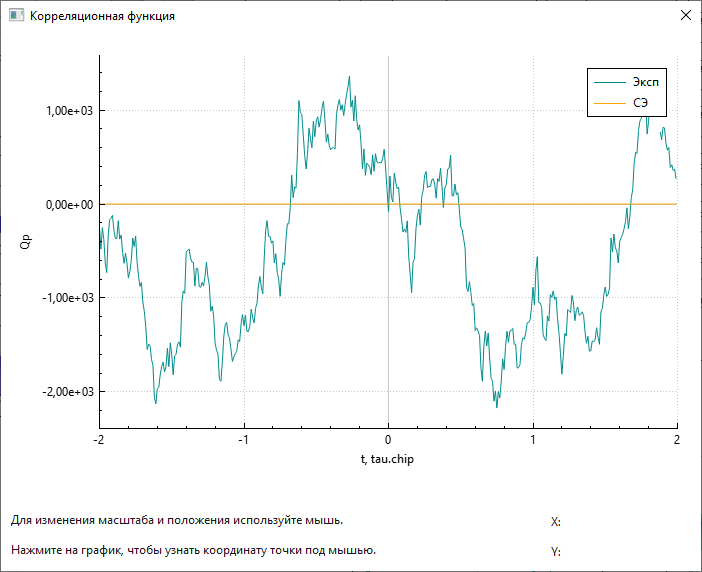
\includegraphics[width=\linewidth]{25_квантбесккор.PNG}
        % \caption*{(б) Квадратурная компонента $Q_p$}
    % \end{minipage}
    % \caption{Корреляционные функции при однобитном квантовании без шума (полоса «Бесконечность»)}
    % \label{fig:quant_corr_inf}
% \end{figure}
% 
% Появление высших гармоник меандра и интермодуляционных искажений при жестком ограничении вызывает изрезанность боковых участков корреляционной функции, однако треугольная форма основного лепестка уверенно сохраняется.
% 
% При совместном действии однобитного компаратора и широкополосного входного шума тепловой шум выступает в качестве естественного псевдослучайного дизеринга (dither). Случайный шум хаотично переводит мгновенный уровень сигнала через нулевой порог квантования компаратора, благодаря чему математическое ожидание бинарной последовательности на выходе АЦП оказывается пропорциональным мгновенному значению аналогового сигнала. Графики корреляционных сумм для условий однобитного квантования в смеси с шумом при полосе $1\text{ МГц}$ представлены на рис.~\ref{fig:quant_noise_1mhz}.
% 
% \begin{figure}[H]
    % \centering
    % \begin{minipage}[b]{0.48\textwidth}
        % \centering
        % 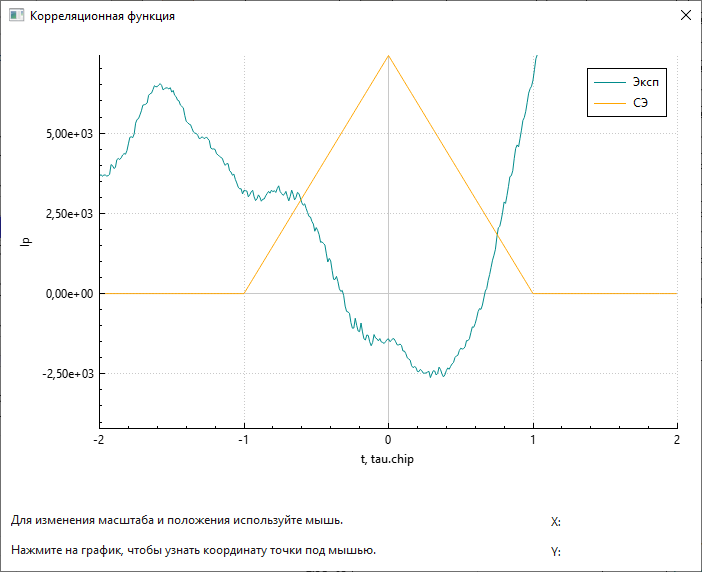
\includegraphics[width=\linewidth]{26)_корплюсшум1.PNG}
        % \caption*{(а) Синфазная компонента $I_p$}
    % \end{minipage}
    % \hfill
    % \begin{minipage}[b]{0.48\textwidth}
        % \centering
        % 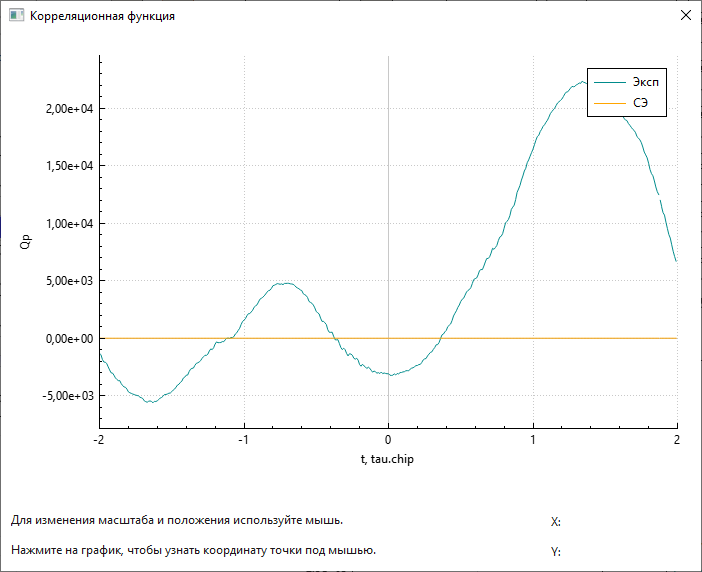
\includegraphics[width=\linewidth]{27_корплюсшум1.PNG}
        % \caption*{(б) Квадратурная компонента $Q_p$}
    % \end{minipage}
    % \caption{Корреляционные функции при однобитном квантовании в смеси с шумом (полоса 1 МГц)}
    % \label{fig:quant_noise_1mhz}
% \end{figure}
% 
% Теоретические потери отношения сигнал/шум при однобитном квантовании на фоне гауссовского шума составляют $10\lg(\pi/2) \approx 1{,}96\text{ дБ}$. Графики подтверждают, что даже при столь радикальном снижении разрядности входного тракта корреляционный канал сохраняет способность к обнаружению сигнала и формированию дискриминационной характеристики, обеспечивая при этом предельную простоту аппаратной реализации умножителей на ПЛИС.
% 
% \subsection{Исследование влияния гармонической помехи}
% 
% На следующем этапе была подключена аддитивная гармоническая узкополосная помеха. Спектральная плотность мощности процесса на выходе фронтенда приведена на рис.~\ref{fig:spec_jamming}.
% 
% \begin{figure}[H]
    % \centering
    % \begin{minipage}[b]{0.48\textwidth}
        % \centering
        % 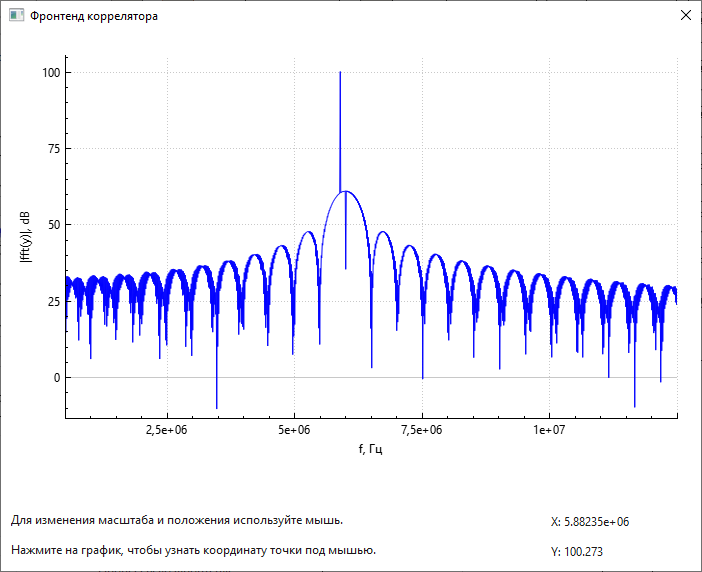
\includegraphics[width=\linewidth]{28_спектрбеск.PNG}
        % \caption*{(а) Обзорный спектр процесса}
    % \end{minipage}
    % \hfill
    % \begin{minipage}[b]{0.48\textwidth}
        % \centering
        % 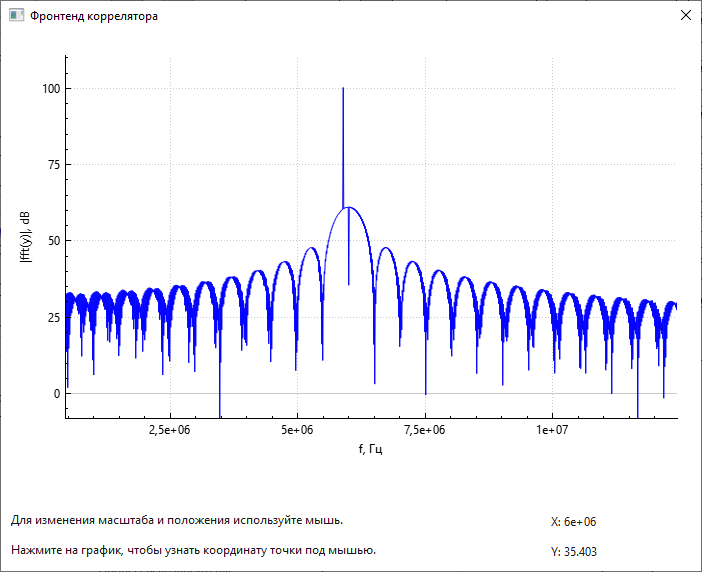
\includegraphics[width=\linewidth]{29_сектрбескпом.PNG}
        % \caption*{(б) Спектр с фиксацией пика помехи}
    % \end{minipage}
    % \caption{Спектральная плотность мощности сигнала в присутствии узкополосной помехи}
    % \label{fig:spec_jamming}
% \end{figure}
% 
% По спектральной диаграмме фиксируется узкополосный всплеск на частоте $f_j \approx 5{,}88\text{ МГц}$ с амплитудой спектральной плотности порядка $100\text{ дБ}$, что существенно превышает спектральный максимум полезного навигационного сигнала ($60\text{ дБ}$). По временной реализации амплитуда помехи составляет $A_j \approx 3{,}9\text{ В}$, откуда мощность помехи оценивается как $P_j = A_j^2 / 2 \approx 7{,}6\text{ Вт}$. Отношение мощности помехи к мощности полезного сигнала составляет $P_j / P_s = 7{,}6 / 0{,}428 \approx 17{,}7$ (около $12{,}5\text{ дБ}$), что соответствует условиям преднамеренного или непреднамеренного радиоэлектронного подавления.
% 
% Несмотря на значительное превышение уровня помехи над уровнем полезного радиосигнала, процедура корреляционной свертки с псевдослучайной последовательностью осуществляет декорреляцию сосредоточенного гармонического колебания. Спектр помехи «размазывается» по полосе ПСП, в то время как энергия полезного сигнала когерентно аккумулируется, подтверждая высокую помехоустойчивость широкополосных навигационных систем.
% 
% \subsection{Исследование процессов в пошаговой регистровой модели аппаратного коррелятора}
% 
% Для детального анализа физических и логических процессов, протекающих в цифровом ядре навигационного приёмника (на базе ПЛИС или специализированной интегральной микросхемы ASIC), была исследована пошаговая регистровая модель квадратурного коррелятора. Данная интерактивная модель воспроизводит конвейерную структуру аппаратного тракта, включающую генератор сетки опорных частот несущей (NCO) с таблицами значений синусов и косинусов (LUT), регистровую линию задержки дальномерного кода с отводами опережающей ($E$), точной ($P$) и запаздывающей ($L$) фаз, а также параллельный массив цифровых умножителей и накапливающих сумматоров (аккумуляторов).
% 
% Первоначально пошаговое продвижение отсчетов с помощью подачи импульсов синхронизации (\texttt{clk}) исследовалось в отсутствие собственного шума приёмника. Окно модели для данного состояния представлено на рис.~\ref{fig:step_clean}.
% 
% \begin{figure}[H]
    % \centering
    % 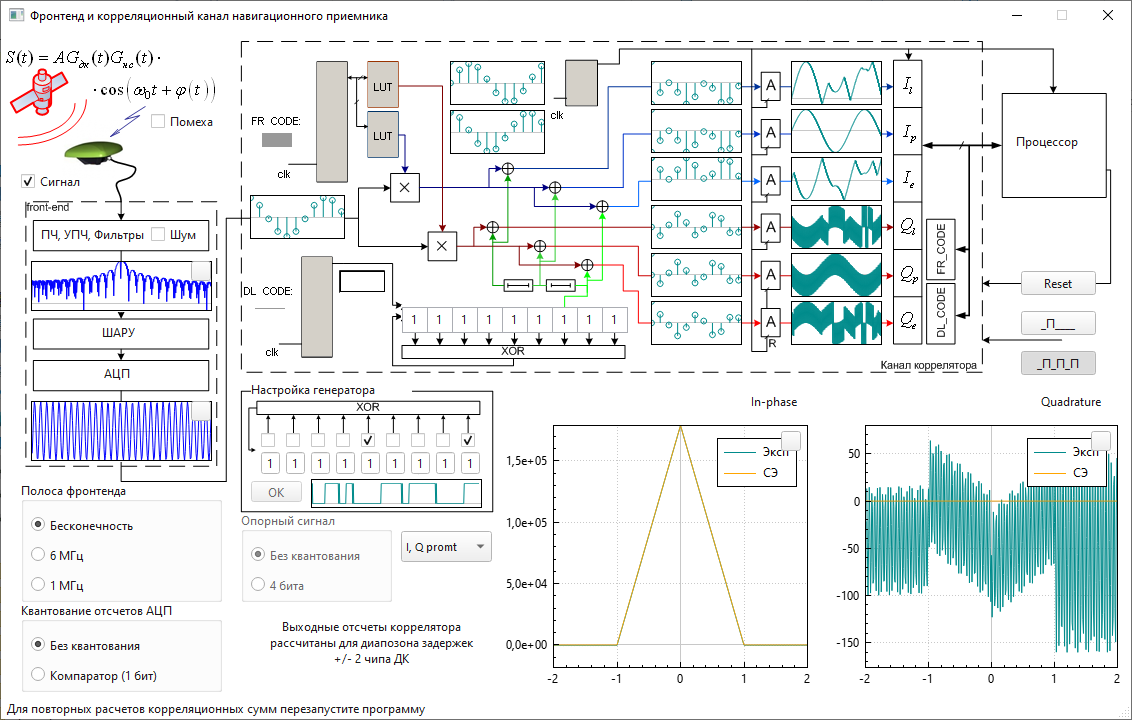
\includegraphics[width=0.85\linewidth]{32.PNG}
    % \caption{Пошаговая регистровая модель коррелятора в отсутствие шума}
    % \label{fig:step_clean}
% \end{figure}
% 
% На схеме отчётливо прослеживается параллельная обработка входных отсчетов: оцифрованный сигнал синхронно перемножается с квадратурными компонентами опорной несущей, после чего сформированные синфазные и квадратурные потоки перемножаются с тремя фазовыми копиями дальномерного кода. Накопление в регистрах аккумуляторов $I_l$, $I_p$, $I_e$ формирует гладкие монотонно нарастающие процессы, причем уровень накопленной суммы в канале $I_p$ достигает максимума при точном совпадении задержки, а каналы $I_e$ и $I_l$ демонстрируют симметричный уровень отклика, необходимый для работы дискриминатора схемы слежения за задержкой. В квадратурных каналах $Q_l$, $Q_p$, $Q_e$ амплитуда накопленного сигнала остаётся близкой к нулю за счёт синфазности опорной несущей с сигналом.
% 
% Далее во входной тракт был введён аддитивный широкополосный шум приёмного устройства. Состояние регистров коррелятора при воздействии шума показано на рис.~\ref{fig:step_noise}.
% 
% \begin{figure}[H]
    % \centering
    % 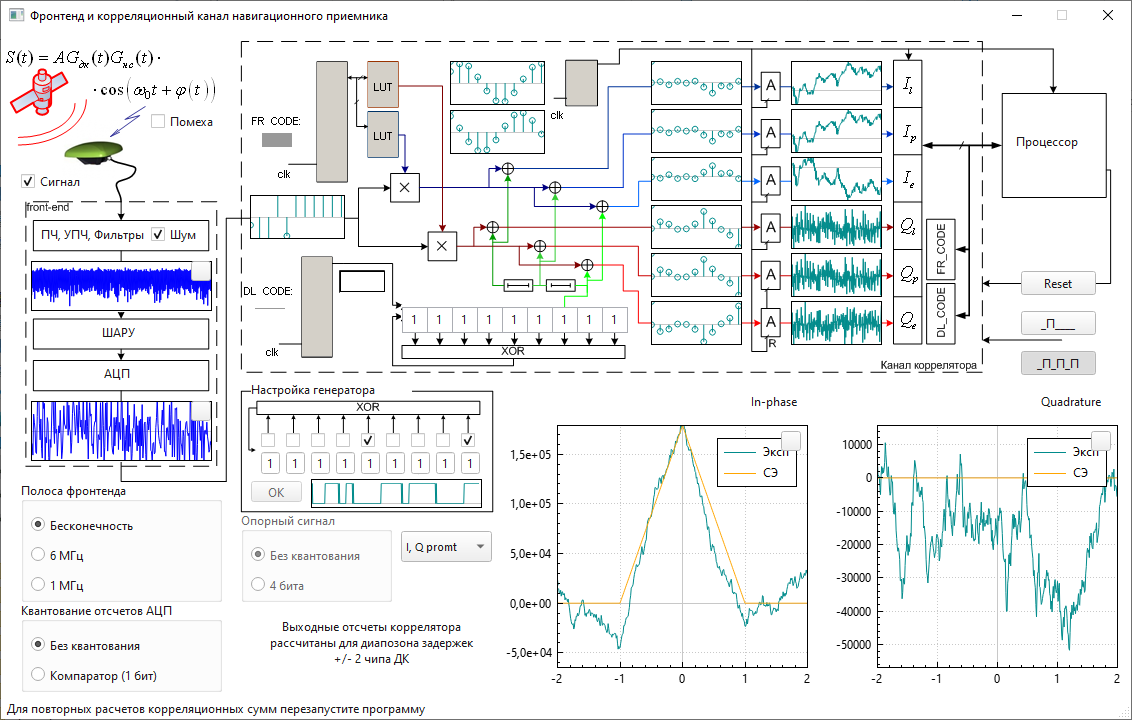
\includegraphics[width=0.85\linewidth]{31_шагпоследний.PNG}
    % \caption{Пошаговая регистровая модель коррелятора при наличии аддитивного шума}
    % \label{fig:step_noise}
% \end{figure}
% 
% Присутствие интенсивного входного шума кардинально меняет характер процессов во внутренних ячейках: выходные отсчёты умножителей приобретают выраженный флуктуационный характер, а кривые накопления в интеграторах представляют собой реализации случайных блужданий с дрейфом. Тем не менее, благодаря когерентному накоплению полезной псевдослучайной последовательности на интервале времени $T = 1\text{ мс}$, детерминированная составляющая сигнала непрерывно суммируется во времени, в то время как некоррелированный шум накапливается по дисперсии пропорционально корню из числа отсчётов. Это обеспечивает уверенное выделение полезного отклика на фоне помех по окончании интервала когерентного накопления перед передачей отсчетов в навигационный процессор.